\documentclass[a4paper, 12pt]{article}

\usepackage{amsmath}
\usepackage[utf8]{inputenc}
\usepackage{graphicx}
\usepackage{caption}
\usepackage{physics}

\captionsetup{width=0.8 \linewidth}

\begin{document}

\title{FFR120 - Homework 2}
\author{Vincent Udén\\udenv@student.chalmers.se}
\date{November - 2022}

\maketitle

\section*{Excercise 7.1}
Following the parameters given in the excercise I obtained the distribution shown in figure \ref{fig:freediff}. For the distributions pictured the numerically calculated standard deviations were $0.99752 \sigma \sqrt{j \Delta t}$, $1.0112 \sigma \sqrt{j \Delta t}$ and $1.0010 \sigma \sqrt{j \Delta t}$. The code for this excercise and the rest of them will be presented at the end of the report.

\begin{figure}[h!]
    \centering
    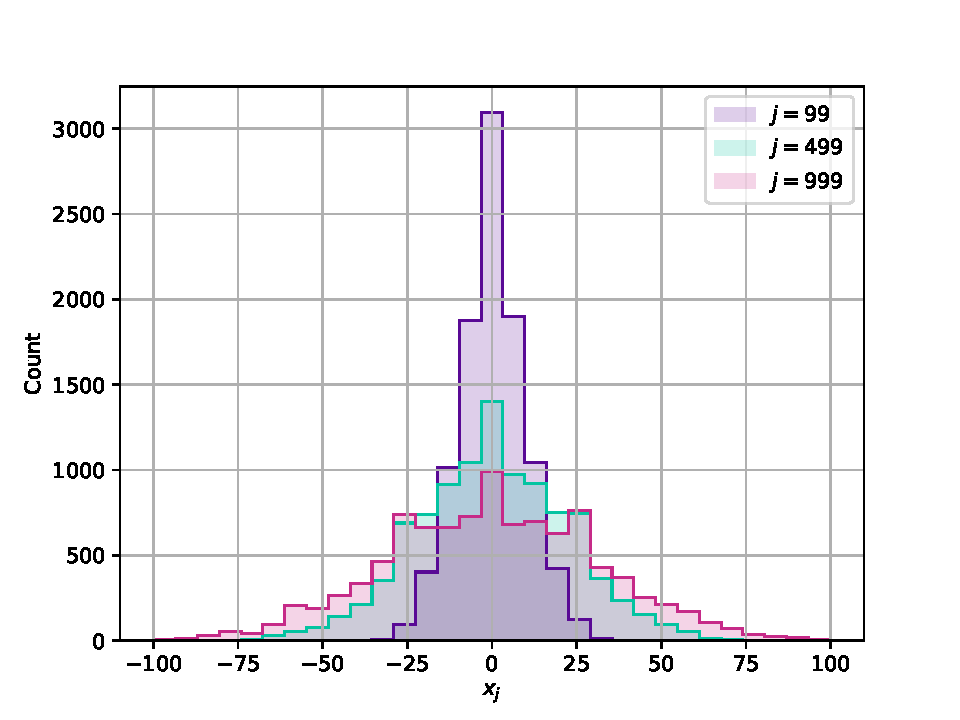
\includegraphics[width=0.8\linewidth]{../Free-Diffusion/free_diff.pdf}
    \caption{Distribution at different times for the free diffusuion of a Brownian particle.}
    \label{fig:freediff}
\end{figure}

\newpage

\section*{Excercise 7.2}
Using the same implementation as previously, adding in reflecting boundary conditions and changing $\Delta t = 0.01\,$s resulted in a program runtime of 5 hours. It turns out that for-loops are extremely slow in Python. Therefore I decided to rewrite the entire thing in C, resulting in a speed up of over 50 times. The resulting distributions are presented below in figure \ref{fig:diffinbox}. It looks very similar to figure 7.3 a) in the book.

\begin{figure}[h!]
    \centering
    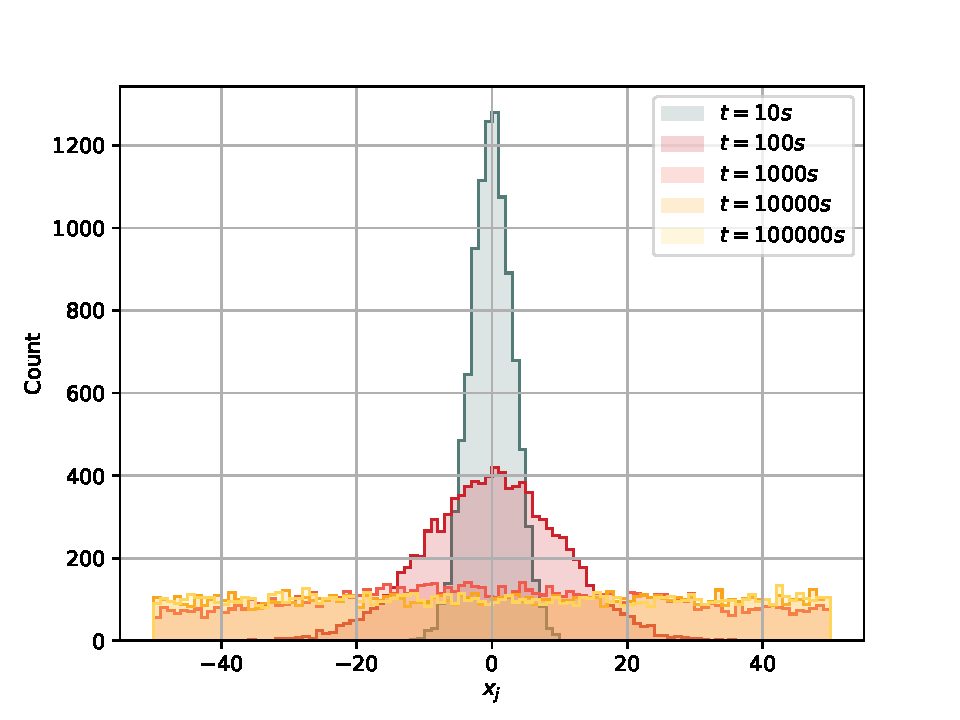
\includegraphics[width=0.8\linewidth]{../Diffusion-In-Box/diffusion-in-box.pdf}
    \caption{Distribution at different times for the diffusuion of a Brownian particle in a one-dimensional box.}
    \label{fig:diffinbox}
\end{figure}

\newpage

\section*{Excercise 7.3}
Using the exact same code as for excercise 7.2, except with a non-constant $\sigma$.

\subsection*{a)}
Using equation 7.7 from the book and the given parameters I obtained the distributions shown in figure \ref{fig:multnoise}.

\begin{figure}[h!]
    \centering
    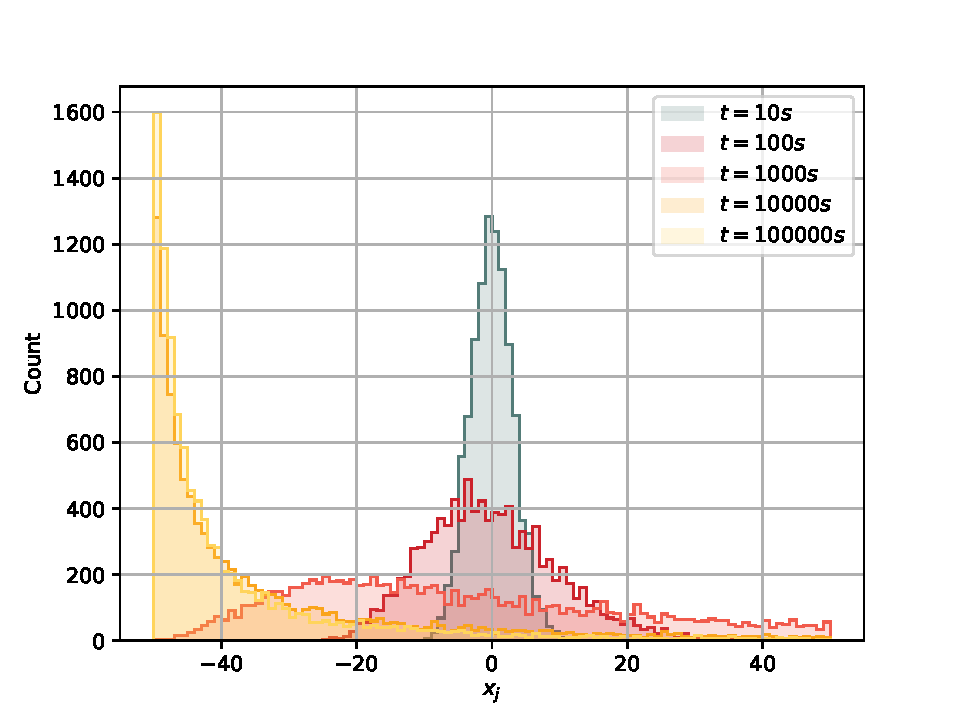
\includegraphics[width=0.8\linewidth]{../Multiplicative-Noise/mult_noise.pdf}
    \caption{Distribution at different times for the diffusuion of a Brownian particle in a one-dimensional box with multiplicative noise.}
    \label{fig:multnoise}
\end{figure}

\subsection*{b)}
Considering the the noise is smaller at the left end, the particles on average gets lower momentum on each update leaving them with a smaller chance of traversing the box rightwards. On the right end of the box, the particles get a lot of momentum. It doesn't matter if this momentum happens to be further rightwards since they'll just reflect off the boundary and head off to the left end. It of course doesn't correspond to what's expected of a physical particle in thermal equilibrium with a system.

\newpage

\section*{Excercise 7.4}
\subsection*{a)}
Using $\alpha = 0.5$ and the noise-induced drift specified in equation 7.11 the following results were obtained as shown in figure \ref{fig:strat}.

\begin{figure}[h!]
    \centering
    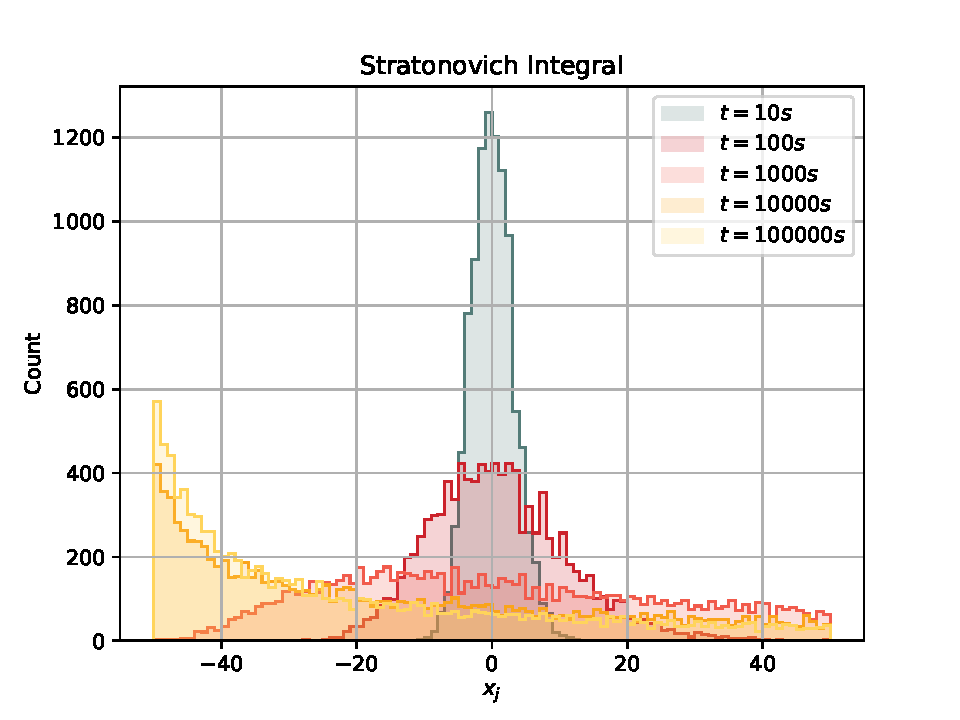
\includegraphics[width=0.8\linewidth]{../Spurious-Drift/stratonovich.pdf}
    \caption{Distribution at different times for the diffusuion of a Brownian particle in a one-dimensional box.}
    \label{fig:strat}
\end{figure}

\subsection*{b)}
When instead computing the anti-Itô integral using $\alpha = 1$ a different distribution is instead computed as is shown in figure \ref{fig:antiito}.

\begin{figure}[h!]
    \centering
    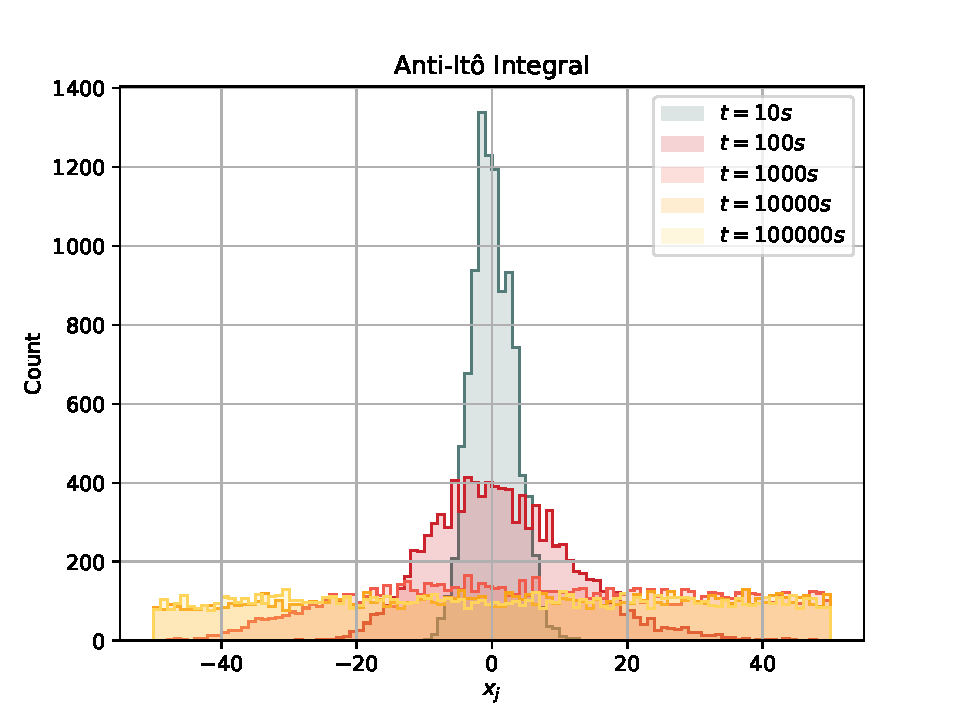
\includegraphics[width=0.8\linewidth]{../Spurious-Drift/anti-ito.pdf}
    \caption{Distribution at different times for the diffusuion of a Brownian particle in a one-dimensional box.}
    \label{fig:antiito}
\end{figure}

\newpage

\subsection*{c)}
Using my results, the Anti-Itô integral seems to produce the best distribution although it is not perfect for my finite but still long timescales. Even for $10^5$ s, it is possible to see a slight bias for the opposite side when compared to the Stratonovich integral. There is a little dip on the left hand side, and the earlier distributions almost look like poission distributions as opposed to Gaussians.

\end{document}
